%%%%%%%%%%%%%%%%%%%%%%%%%%%%%%%%%%%
\chapter{Comparação entre Membros e Não Membros}\label{apendice:comparacao_nucleo}
%%%%%%%%%%%%%%%%%%%%%%%%%%%%%%%%%%%

\begin{figure}[!htb]
  \begin{center}
  \subfloat[Coeficiente de agrupamento]{%
    \label{fig:core_com_ccs_clustering_coefficient_apendice}
    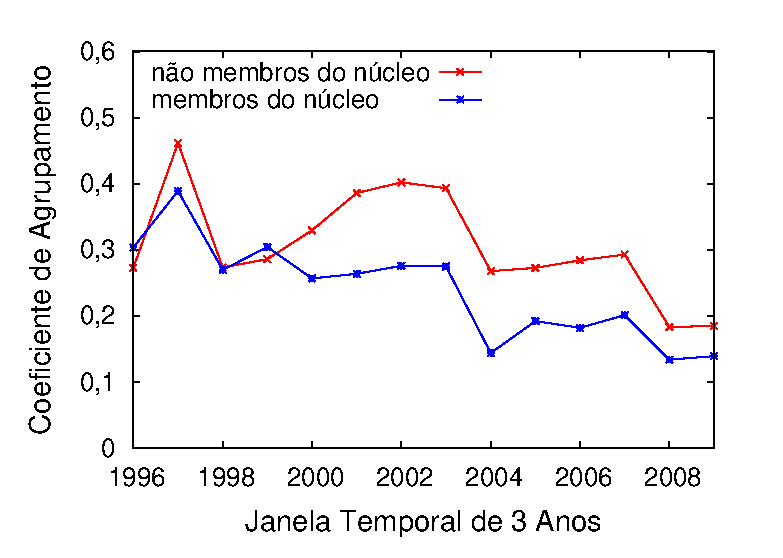
\includegraphics[scale=.6]{../graficos/core_over_time/core_community/pt_BR/ccs_janela_3_core_coeficiente_agrupamento.eps}
  }
  \subfloat[Grau médio]{%
    \label{fig:core_com_ccs_average_degree_apendice}
    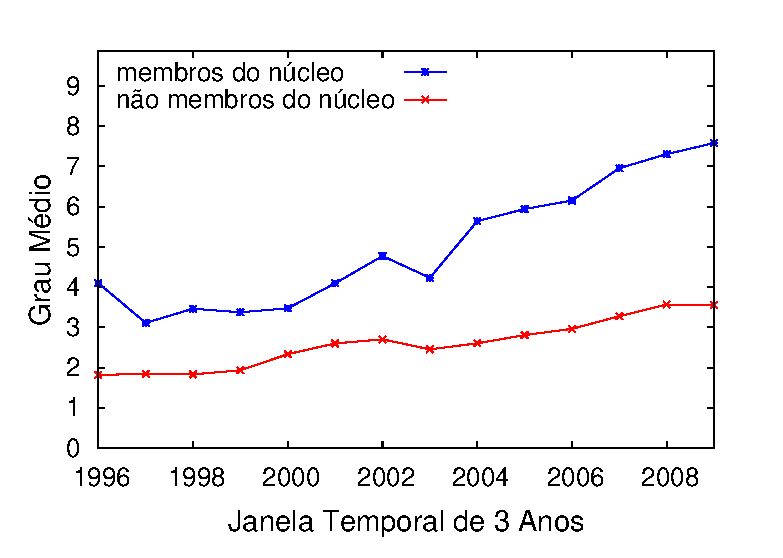
\includegraphics[scale=.6]{../graficos/core_over_time/core_community/pt_BR/ccs_janela_3_core_grau_medio_nodos.eps}
  }
  \phantomcaption
  \end{center}
\end{figure}
\begin{figure}[!htb]
  \begin{center}
  \ContinuedFloat
  \subfloat[Maior CFC]{%
    \label{fig:core_com_ccs_largest_connected_component_apendice}
    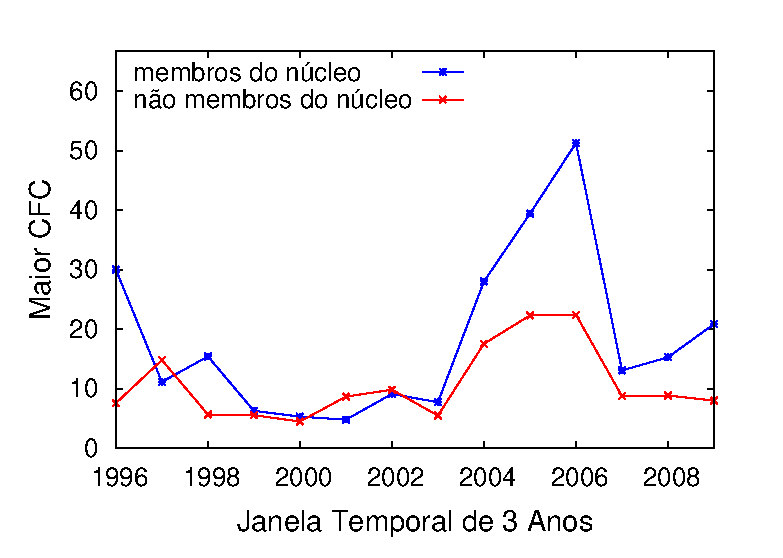
\includegraphics[scale=.6]{../graficos/core_over_time/core_community/pt_BR/ccs_janela_3_core_maior_componente_conectado.eps}
  }
  \subfloat[\textit{Betweenness} médio]{%
    \label{fig:core_com_ccs_betweenness_apendice}
    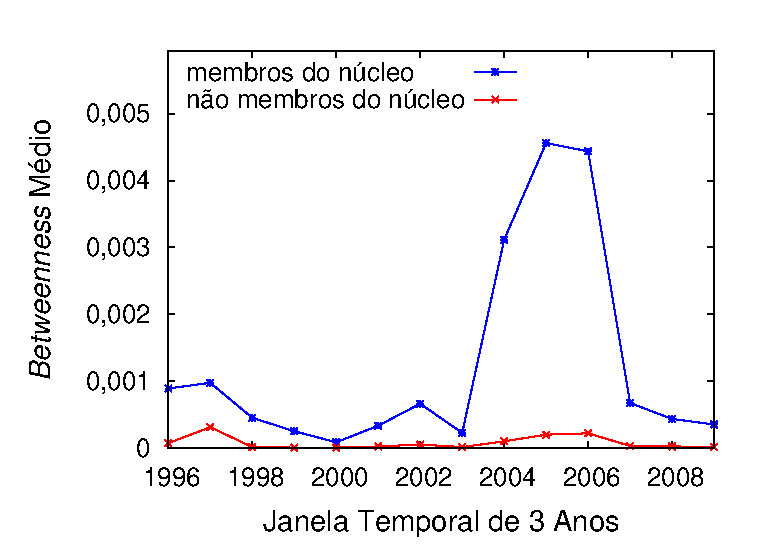
\includegraphics[scale=.6]{../graficos/core_over_time/core_community/pt_BR/ccs_janela_3_core_betweenness.eps}
  }
  \end{center}
  \caption{Propriedades da comunidade CCS para os membros e não membros do núcleo}
  \label{fig:metrics_comparing_core_community_ccs_apendice}
\end{figure}

\begin{figure}[!htb]
  \begin{center}
  \subfloat[Coeficiente de agrupamento]{%
    \label{fig:core_com_chi_clustering_coefficient_apendice}
    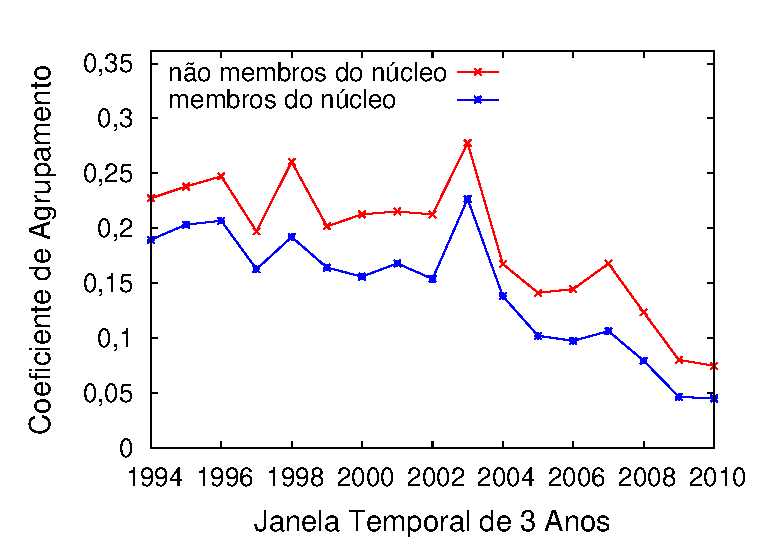
\includegraphics[scale=.6]{../graficos/core_over_time/core_community/pt_BR/chi_janela_3_core_coeficiente_agrupamento.eps}
  }
  \subfloat[Grau médio]{%
    \label{fig:core_com_chi_average_degree_apendice}
    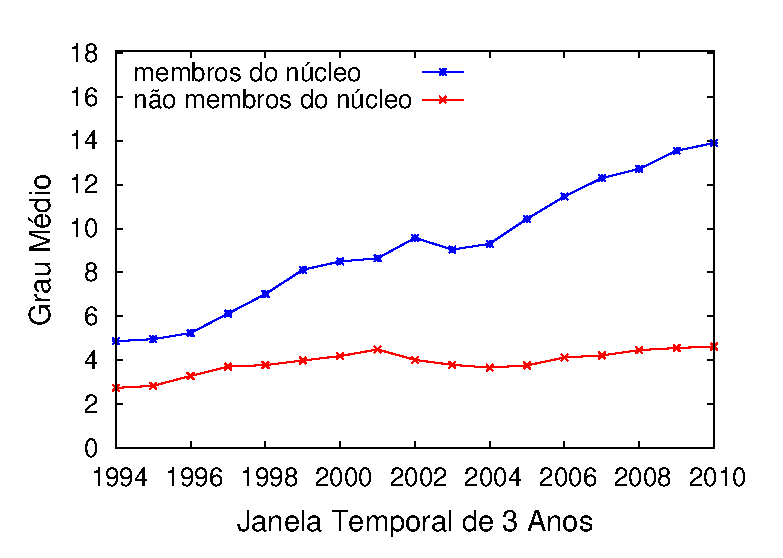
\includegraphics[scale=.6]{../graficos/core_over_time/core_community/pt_BR/chi_janela_3_core_grau_medio_nodos.eps}
  }
  \\
  \subfloat[Maior CFC]{%
    \label{fig:core_com_chi_largest_connected_component_apendice}
    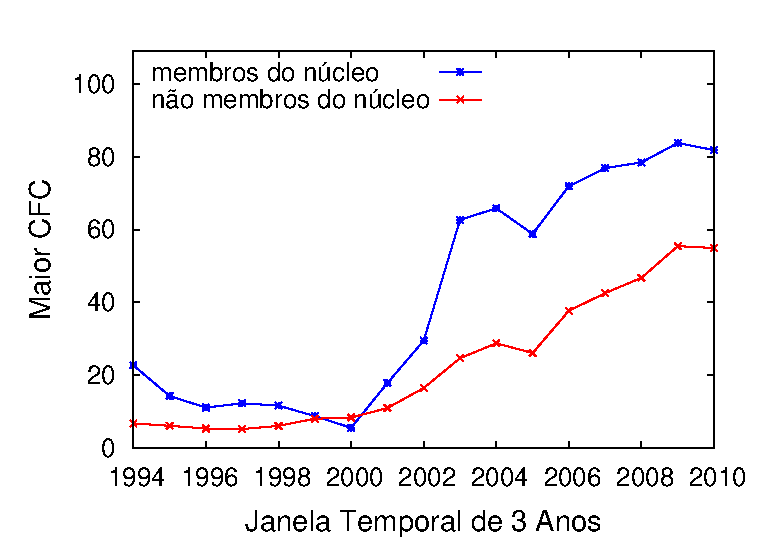
\includegraphics[scale=.6]{../graficos/core_over_time/core_community/pt_BR/chi_janela_3_core_maior_componente_conectado.eps}
  }
  \subfloat[\textit{Betweenness} médio]{%
    \label{fig:core_com_chi_betweenness_apendice}
    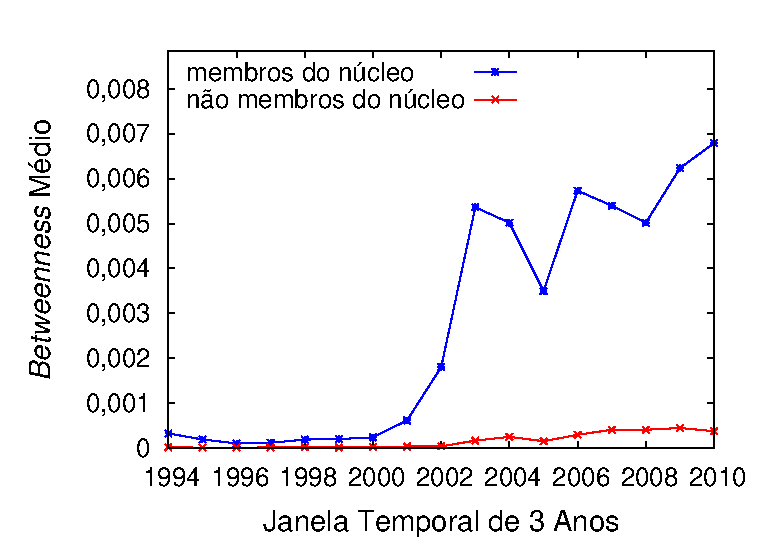
\includegraphics[scale=.6]{../graficos/core_over_time/core_community/pt_BR/chi_janela_3_core_betweenness.eps}
  }
  \end{center}
  \caption{Propriedades da comunidade CHI para os membros e não membros do núcleo}
  \label{fig:metrics_comparing_core_community_chi_apendice}
\end{figure}

\begin{figure}[!htb]
  \begin{center}
  \subfloat[Coeficiente de agrupamento]{%
    \label{fig:core_com_cikm_clustering_coefficient_apendice}
    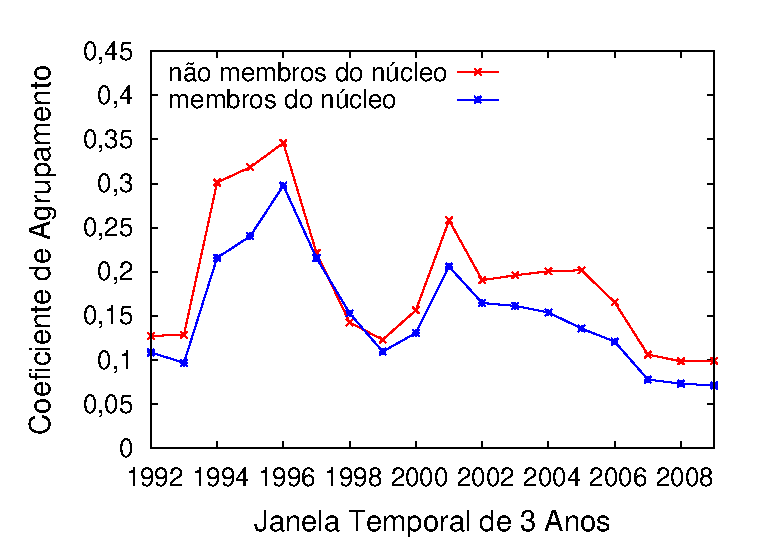
\includegraphics[scale=.6]{../graficos/core_over_time/core_community/pt_BR/cikm_janela_3_core_coeficiente_agrupamento.eps}
  }
  \subfloat[Grau médio]{%
    \label{fig:core_com_cikm_average_degree_apendice}
    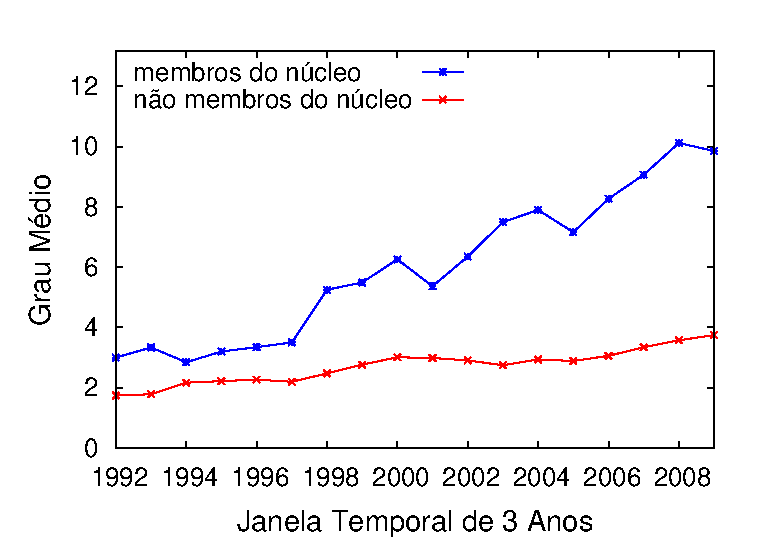
\includegraphics[scale=.6]{../graficos/core_over_time/core_community/pt_BR/cikm_janela_3_core_grau_medio_nodos.eps}
  }
  \\
  \subfloat[Maior CFC]{%
    \label{fig:core_com_cikm_largest_connected_component_apendice}
    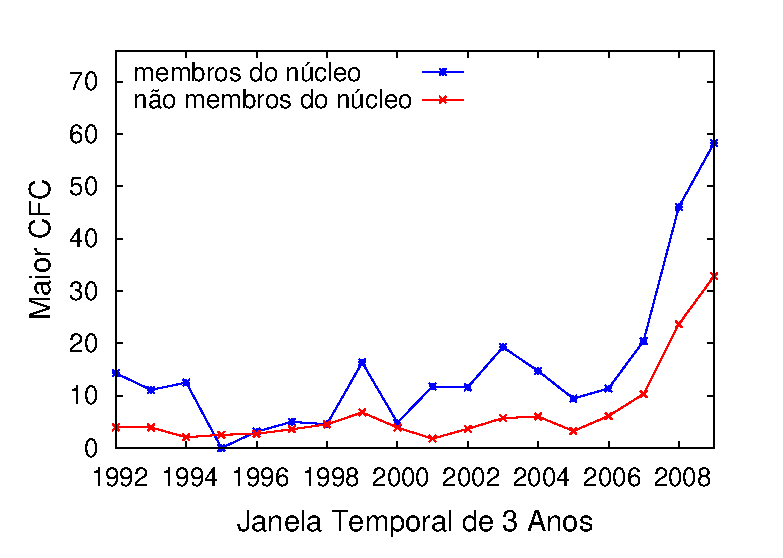
\includegraphics[scale=.6]{../graficos/core_over_time/core_community/pt_BR/cikm_janela_3_core_maior_componente_conectado.eps}
  }
  \subfloat[\textit{Betweenness} médio]{%
    \label{fig:core_com_cikm_betweenness_apendice}
    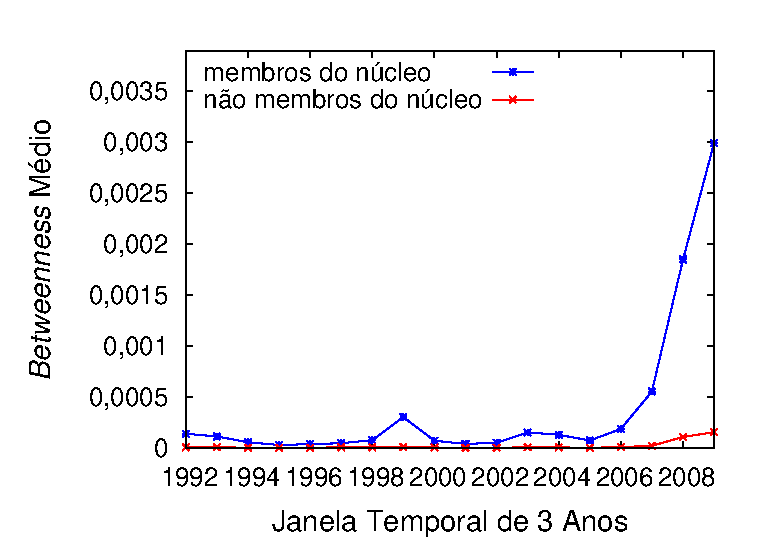
\includegraphics[scale=.6]{../graficos/core_over_time/core_community/pt_BR/cikm_janela_3_core_betweenness.eps}
  }
  \end{center}
  \caption{Propriedades da comunidade CIKM para os membros e não membros do núcleo}
  \label{fig:metrics_comparing_core_community_cikm_apendice}
\end{figure}

\begin{figure}[!htb]
  \begin{center}
  \subfloat[Coeficiente de agrupamento]{%
    \label{fig:core_com_dac_clustering_coefficient_apendice}
    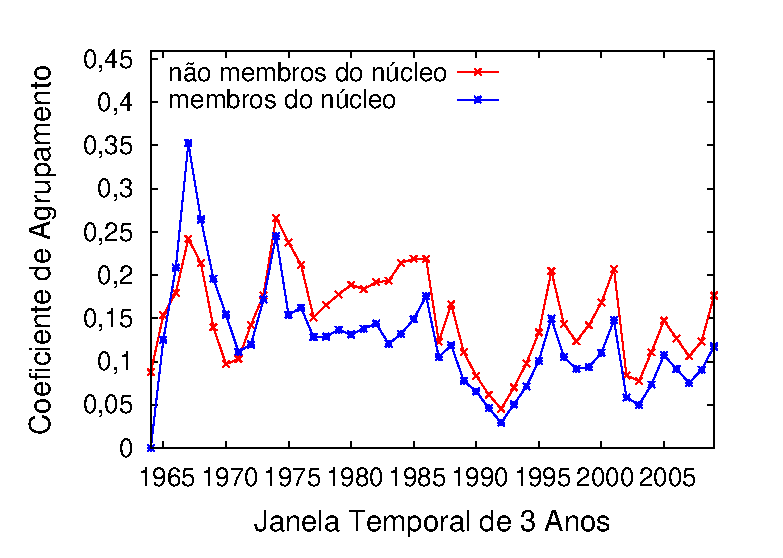
\includegraphics[scale=.6]{../graficos/core_over_time/core_community/pt_BR/dac_janela_3_core_coeficiente_agrupamento.eps}
  }
  \subfloat[Grau médio]{%
    \label{fig:core_com_dac_average_degree_apendice}
    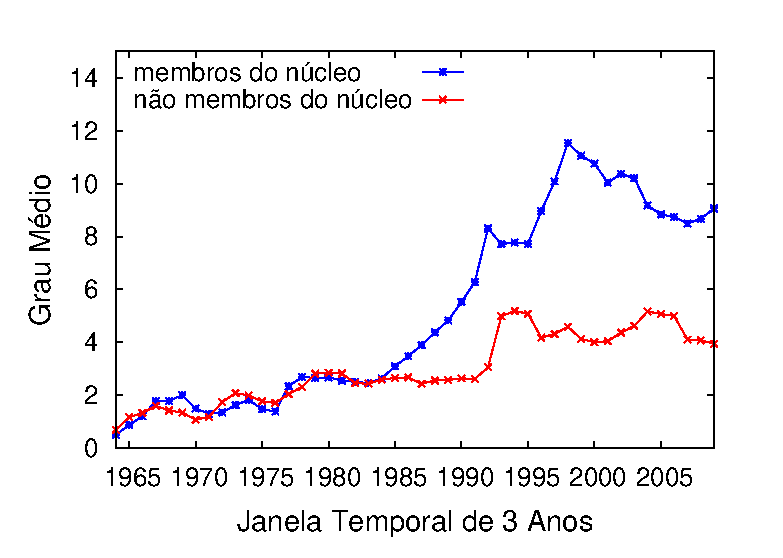
\includegraphics[scale=.6]{../graficos/core_over_time/core_community/pt_BR/dac_janela_3_core_grau_medio_nodos.eps}
  }
\phantomcaption
  \end{center}
\end{figure}
\begin{figure}[!htb]
  \begin{center}
  \ContinuedFloat
  \subfloat[Maior CFC]{%
    \label{fig:core_com_dac_largest_connected_component_apendice}
    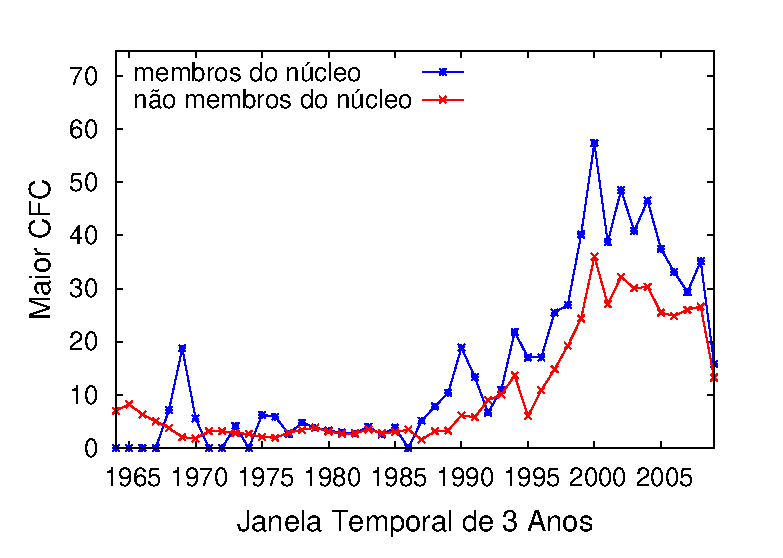
\includegraphics[scale=.6]{../graficos/core_over_time/core_community/pt_BR/dac_janela_3_core_maior_componente_conectado.eps}
  }
  \subfloat[\textit{Betweenness} médio]{%
    \label{fig:core_com_dac_betweenness_apendice}
    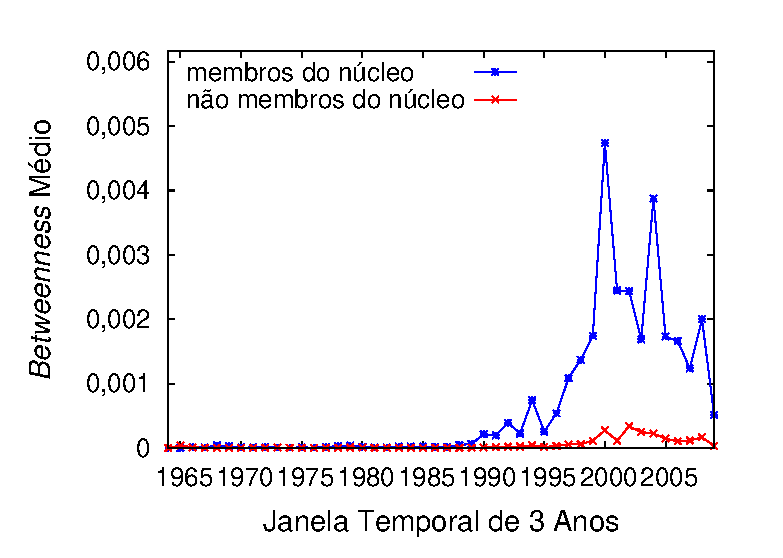
\includegraphics[scale=.6]{../graficos/core_over_time/core_community/pt_BR/dac_janela_3_core_betweenness.eps}
  }
  \end{center}
  \caption{Propriedades da comunidade DAC para os membros e não membros do núcleo}
  \label{fig:metrics_comparing_core_community_dac_apendice}
\end{figure}

\begin{figure}[!htb]
  \begin{center}
  \subfloat[Coeficiente de agrupamento]{%
    \label{fig:core_com_hscc_clustering_coefficient_apendice}
    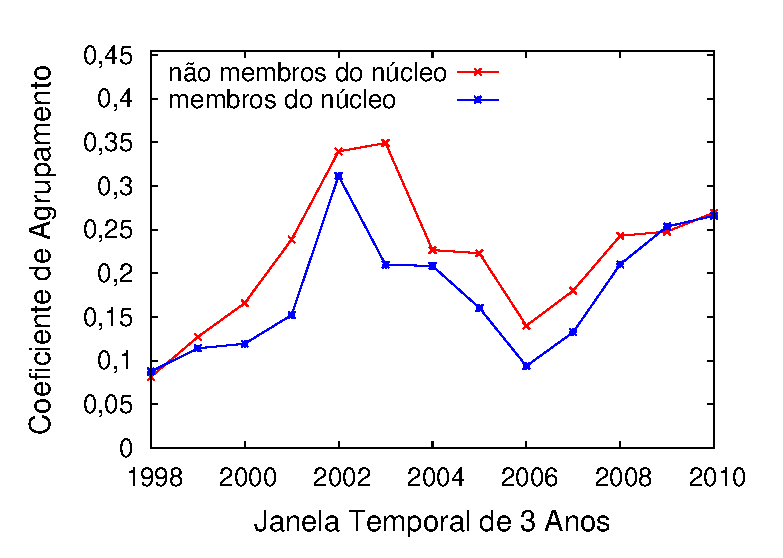
\includegraphics[scale=.6]{../graficos/core_over_time/core_community/pt_BR/hscc_janela_3_core_coeficiente_agrupamento.eps}
  }
  \subfloat[Grau médio]{%
    \label{fig:core_com_hscc_average_degree_apendice}
    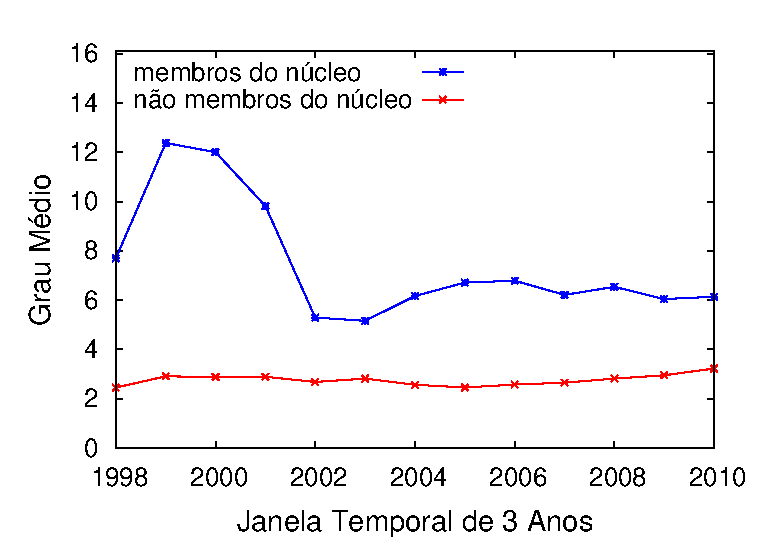
\includegraphics[scale=.6]{../graficos/core_over_time/core_community/pt_BR/hscc_janela_3_core_grau_medio_nodos.eps}
  }
  \\
  \subfloat[Maior CFC]{%
    \label{fig:core_com_hscc_largest_connected_component_apendice}
    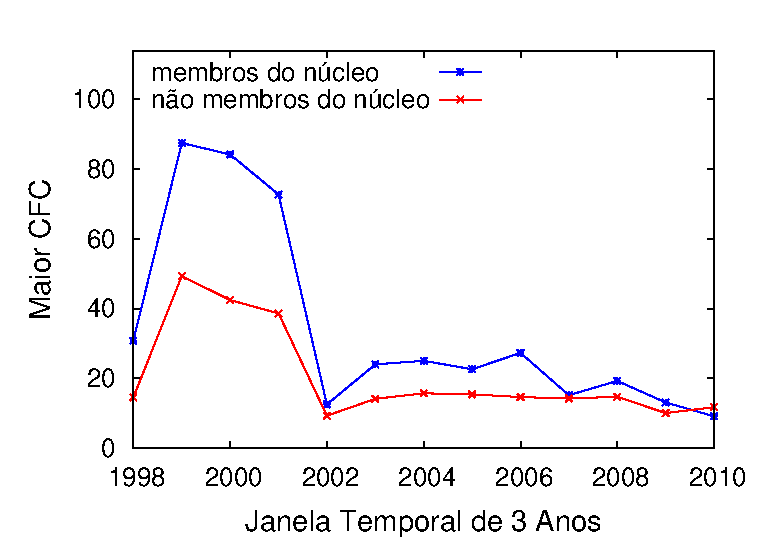
\includegraphics[scale=.6]{../graficos/core_over_time/core_community/pt_BR/hscc_janela_3_core_maior_componente_conectado.eps}
  }
  \subfloat[\textit{Betweenness} médio]{%
    \label{fig:core_com_hscc_betweenness_apendice}
    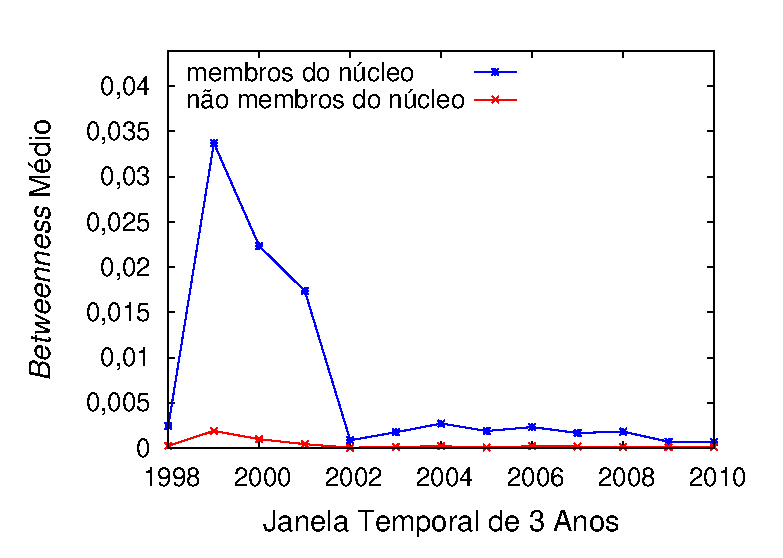
\includegraphics[scale=.6]{../graficos/core_over_time/core_community/pt_BR/hscc_janela_3_core_betweenness.eps}
  }
  \end{center}
  \caption{Propriedades da comunidade HSCC para os membros e não membros do núcleo}
  \label{fig:metrics_comparing_core_community_hscc_apendice}
\end{figure}

\begin{figure}[!htb]
  \begin{center}
  \subfloat[Coeficiente de agrupamento]{%
    \label{fig:core_com_icse_clustering_coefficient_apendice}
    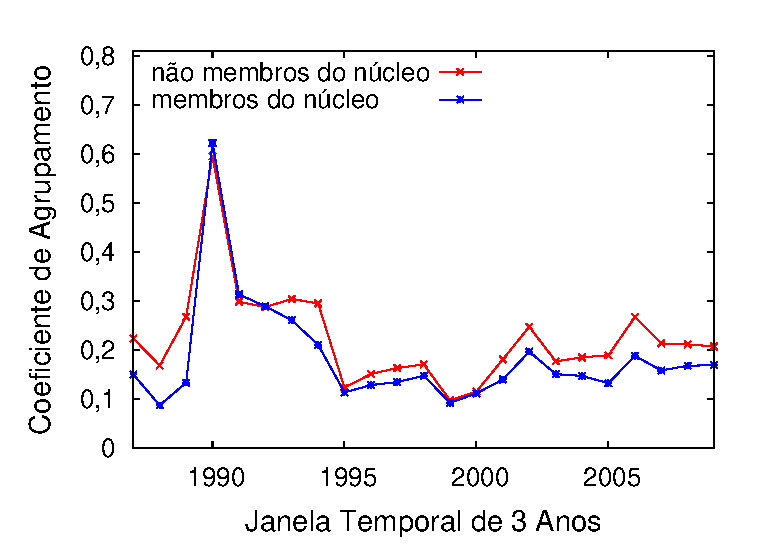
\includegraphics[scale=.6]{../graficos/core_over_time/core_community/pt_BR/icse_janela_3_core_coeficiente_agrupamento.eps}
  }
  \subfloat[Grau médio]{%
    \label{fig:core_com_icse_average_degree_apendice}
    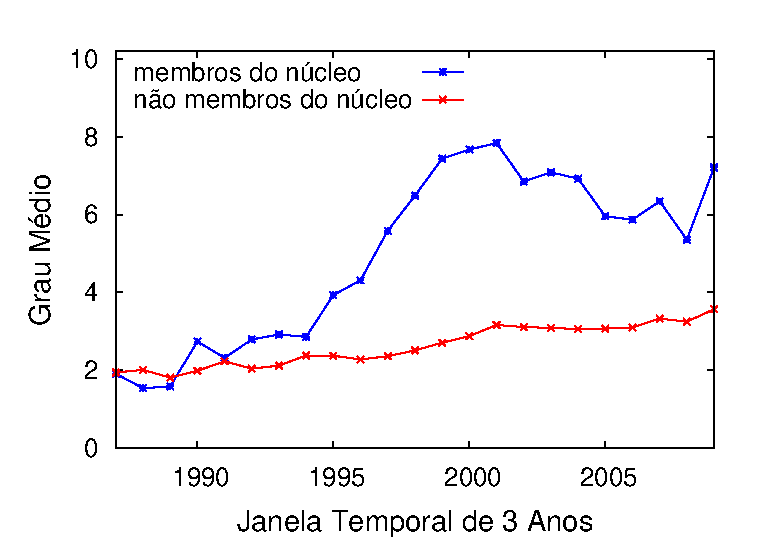
\includegraphics[scale=.6]{../graficos/core_over_time/core_community/pt_BR/icse_janela_3_core_grau_medio_nodos.eps}
  }
  \\
  \subfloat[Maior CFC]{%
    \label{fig:core_com_icse_largest_connected_component_apendice}
    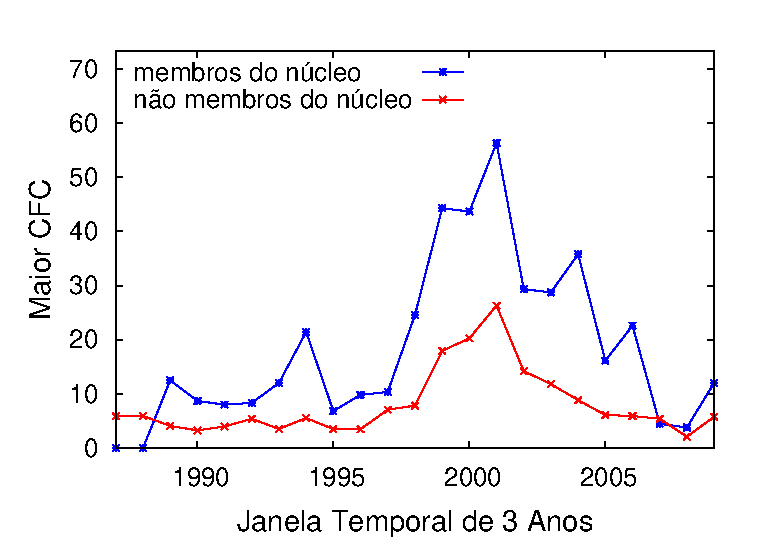
\includegraphics[scale=.6]{../graficos/core_over_time/core_community/pt_BR/icse_janela_3_core_maior_componente_conectado.eps}
  }
  \subfloat[\textit{Betweenness} médio]{%
    \label{fig:core_com_icse_betweenness_apendice}
    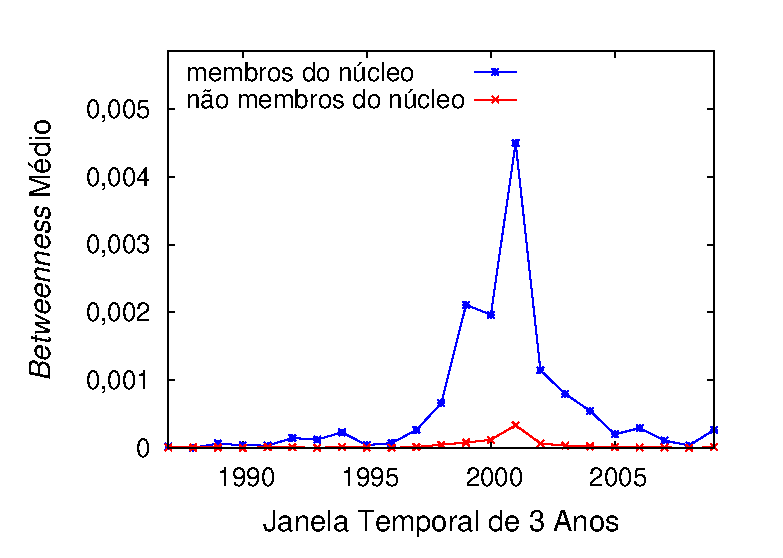
\includegraphics[scale=.6]{../graficos/core_over_time/core_community/pt_BR/icse_janela_3_core_betweenness.eps}
  }
  \end{center}
  \caption{Propriedades da comunidade ICSE para os membros e não membros do núcleo}
  \label{fig:metrics_comparing_core_community_icse_apendice}
\end{figure}

\begin{figure}[!htb]
  \begin{center}
  \subfloat[Coeficiente de agrupamento]{%
    \label{fig:core_com_isca_clustering_coefficient_apendice}
    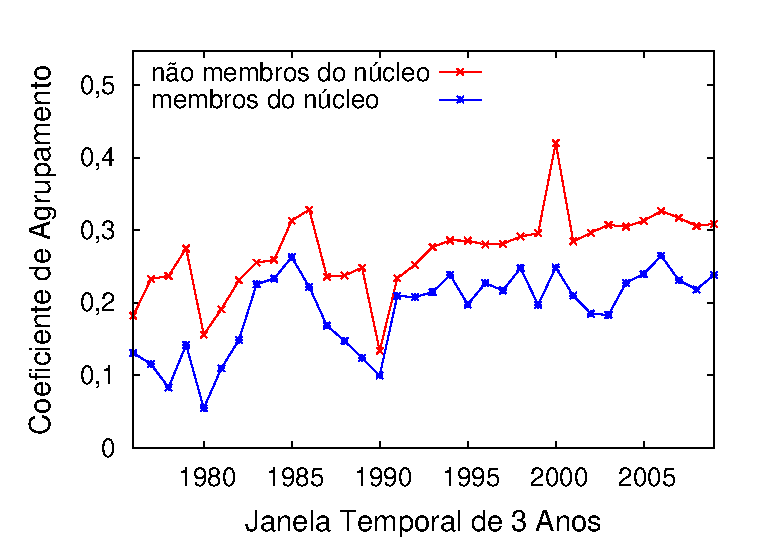
\includegraphics[scale=.6]{../graficos/core_over_time/core_community/pt_BR/isca_janela_3_core_coeficiente_agrupamento.eps}
  }
  \subfloat[Grau médio]{%
    \label{fig:core_com_isca_average_degree_apendice}
    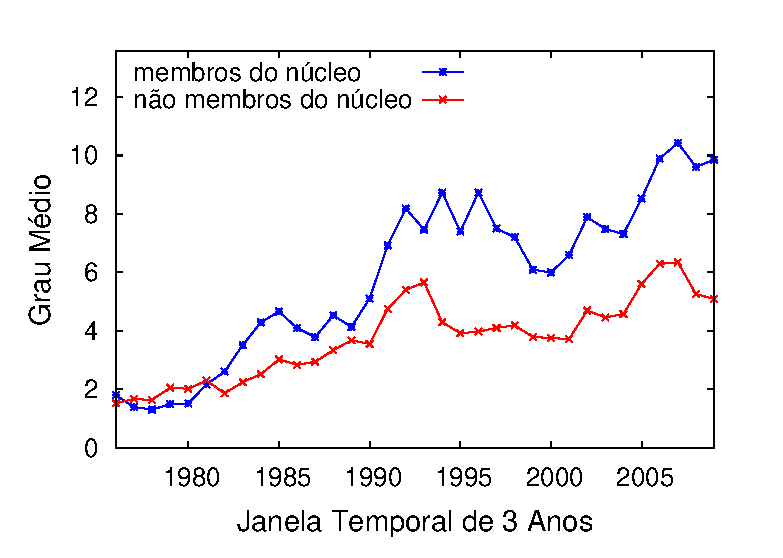
\includegraphics[scale=.6]{../graficos/core_over_time/core_community/pt_BR/isca_janela_3_core_grau_medio_nodos.eps}
  }
  \phantomcaption
  \end{center}
\end{figure}
\begin{figure}[!htb]
  \begin{center}
  \ContinuedFloat
  \subfloat[Maior CFC]{%
    \label{fig:core_com_isca_largest_connected_component_apendice}
    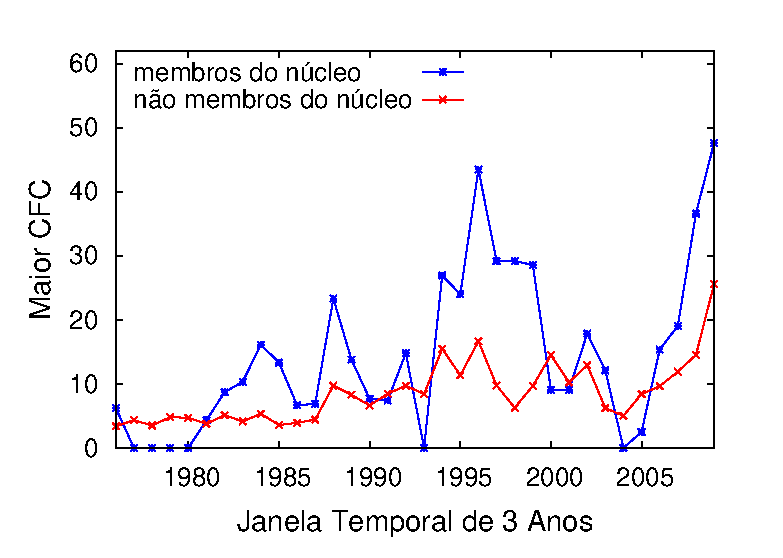
\includegraphics[scale=.6]{../graficos/core_over_time/core_community/pt_BR/isca_janela_3_core_maior_componente_conectado.eps}
  }
  \subfloat[\textit{Betweenness} médio]{%
    \label{fig:core_com_isca_betweenness_apendice}
    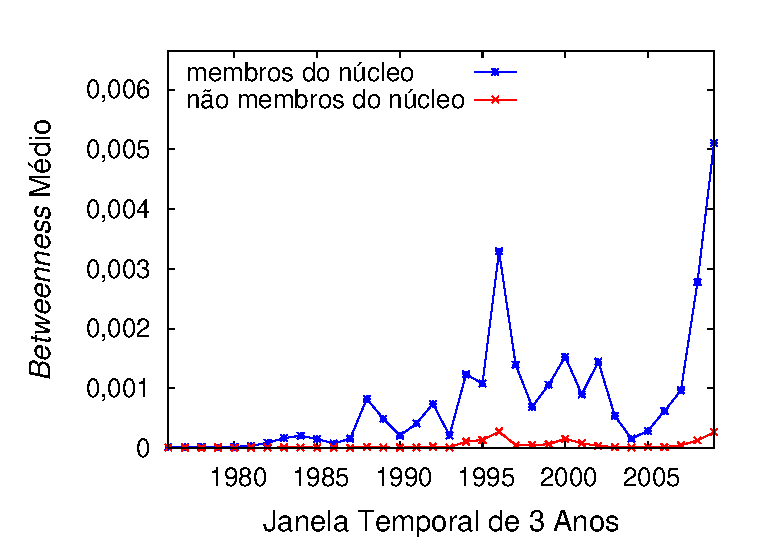
\includegraphics[scale=.6]{../graficos/core_over_time/core_community/pt_BR/isca_janela_3_core_betweenness.eps}
  }
  \end{center}
  \caption{Propriedades da comunidade ISCA para os membros e não membros do núcleo}
  \label{fig:metrics_comparing_core_community_isca_apendice}
\end{figure}

\begin{figure}[!htb]
  \begin{center}
  \subfloat[Coeficiente de agrupamento]{%
    \label{fig:core_com_kdd_clustering_coefficient_apendice}
    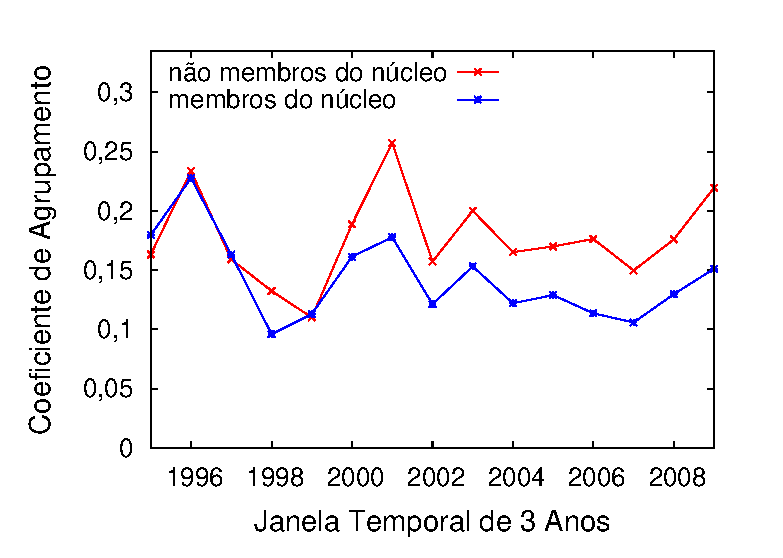
\includegraphics[scale=.6]{../graficos/core_over_time/core_community/pt_BR/kdd_janela_3_core_coeficiente_agrupamento.eps}
  }
  \subfloat[Grau médio]{%
    \label{fig:core_com_kdd_average_degree_apendice}
    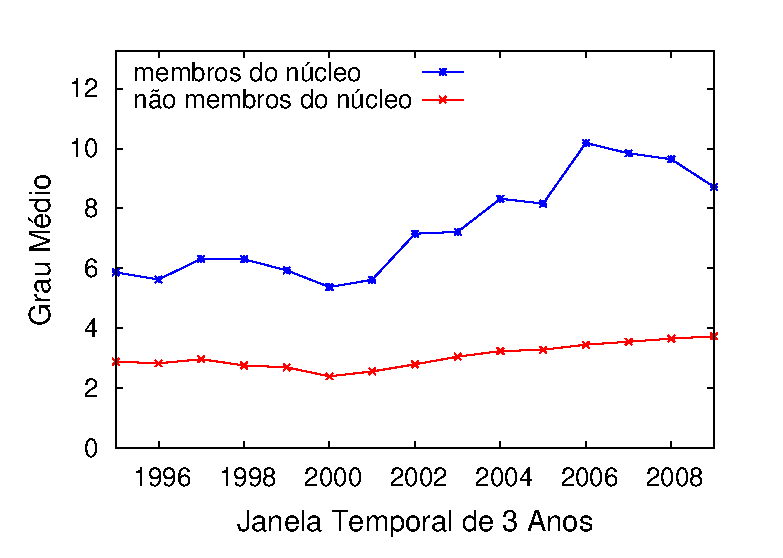
\includegraphics[scale=.6]{../graficos/core_over_time/core_community/pt_BR/kdd_janela_3_core_grau_medio_nodos.eps}
  }
  \\
  \subfloat[Maior CFC]{%
    \label{fig:core_com_kdd_largest_connected_component_apendice}
    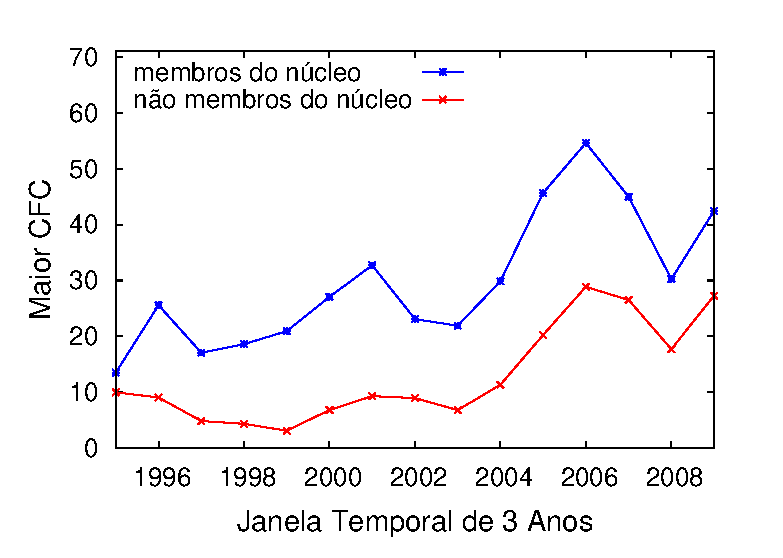
\includegraphics[scale=.6]{../graficos/core_over_time/core_community/pt_BR/kdd_janela_3_core_maior_componente_conectado.eps}
  }
  \subfloat[\textit{Betweenness} médio]{%
    \label{fig:core_com_kdd_betweenness_apendice}
    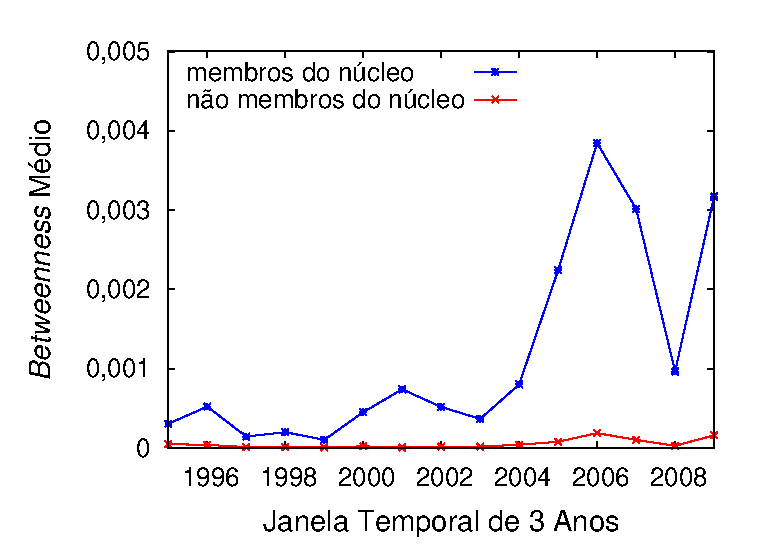
\includegraphics[scale=.6]{../graficos/core_over_time/core_community/pt_BR/kdd_janela_3_core_betweenness.eps}
  }
  \end{center}
  \caption{Propriedades da comunidade KDD para os membros e não membros do núcleo}
  \label{fig:metrics_comparing_core_community_kdd_apendice}
\end{figure}

\begin{figure}[!htb]
  \begin{center}
  \subfloat[Coeficiente de agrupamento]{%
    \label{fig:core_com_micro_clustering_coefficient_apendice}
    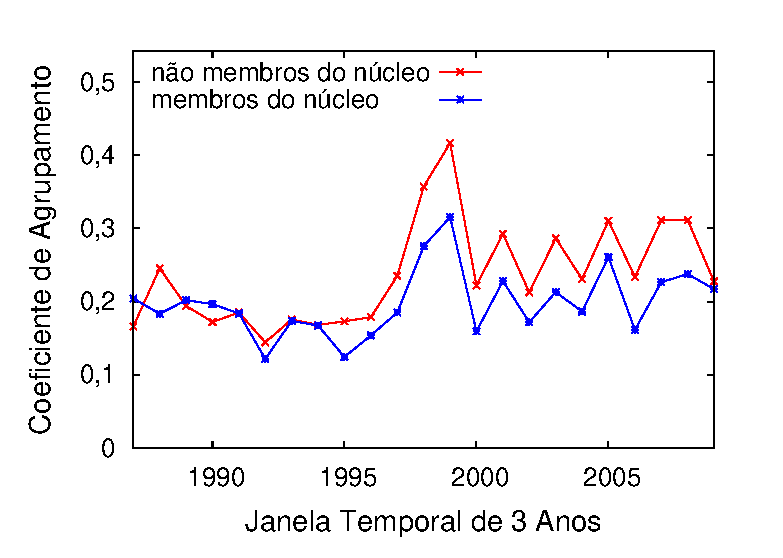
\includegraphics[scale=.6]{../graficos/core_over_time/core_community/pt_BR/micro_janela_3_core_coeficiente_agrupamento.eps}
  }
  \subfloat[Grau médio]{%
    \label{fig:core_com_micro_average_degree_apendice}
    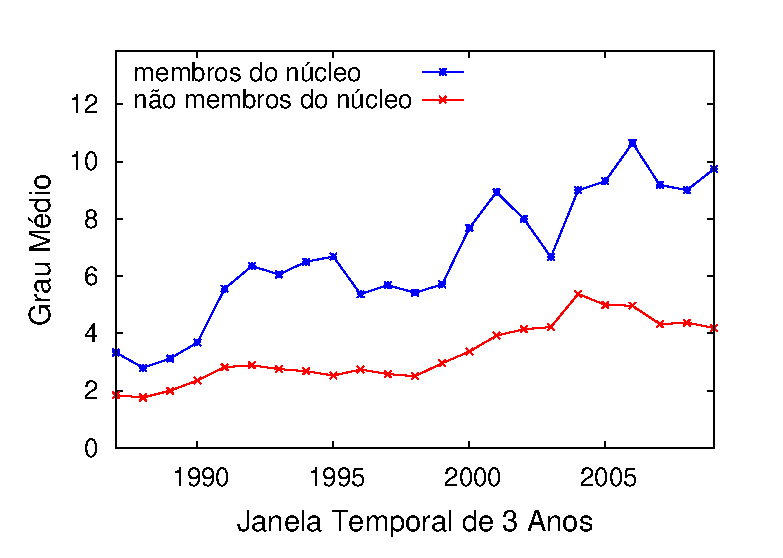
\includegraphics[scale=.6]{../graficos/core_over_time/core_community/pt_BR/micro_janela_3_core_grau_medio_nodos.eps}
  }
  \\
  \subfloat[Maior CFC]{%
    \label{fig:core_com_micro_largest_connected_component_apendice}
    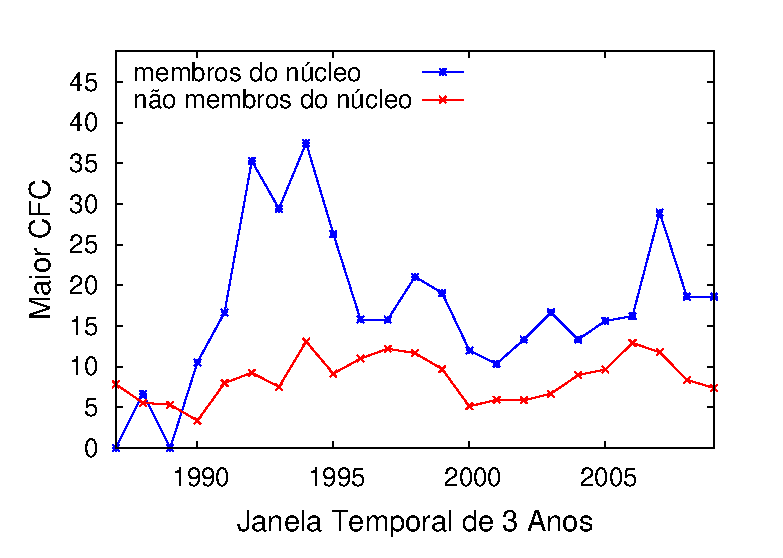
\includegraphics[scale=.6]{../graficos/core_over_time/core_community/pt_BR/micro_janela_3_core_maior_componente_conectado.eps}
  }
  \subfloat[\textit{Betweenness} médio]{%
    \label{fig:core_com_micro_betweenness_apendice}
    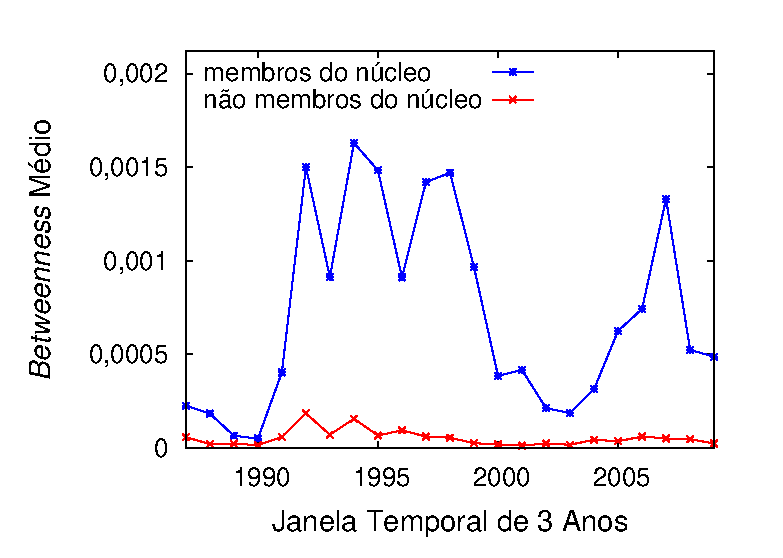
\includegraphics[scale=.6]{../graficos/core_over_time/core_community/pt_BR/micro_janela_3_core_betweenness.eps}
  }
  \end{center}
  \caption{Propriedades da comunidade MICRO para os membros e não membros do núcleo}
  \label{fig:metrics_comparing_core_community_micro_apendice}
\end{figure}

\begin{figure}[!htb]
  \begin{center}
  \subfloat[Coeficiente de agrupamento]{%
    \label{fig:core_com_acm_multimedia_clustering_coefficient_apendice}
    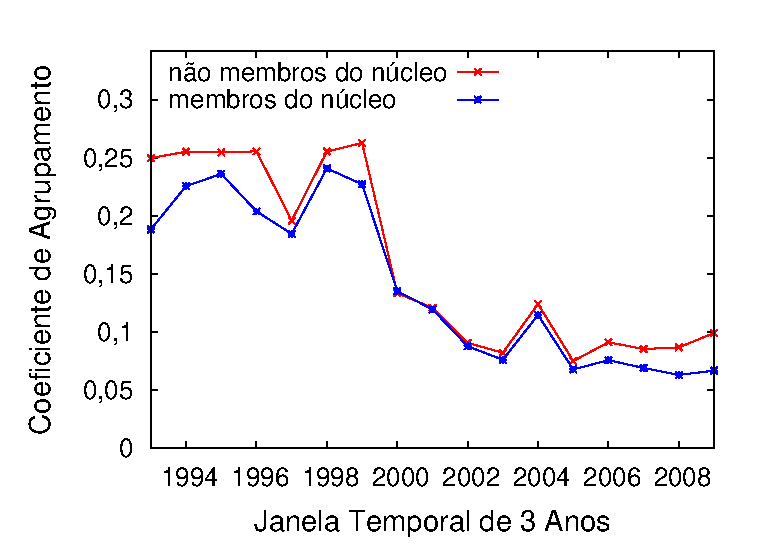
\includegraphics[scale=.6]{../graficos/core_over_time/core_community/pt_BR/acm_multimedia_janela_3_core_coeficiente_agrupamento.eps}
  }
  \subfloat[Grau médio]{%
    \label{fig:core_com_acm_multimedia_average_degree_apendice}
    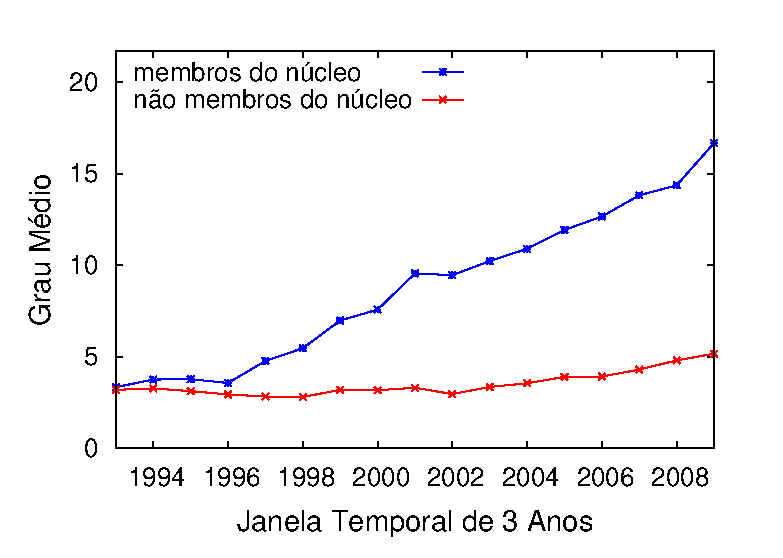
\includegraphics[scale=.6]{../graficos/core_over_time/core_community/pt_BR/acm_multimedia_janela_3_core_grau_medio_nodos.eps}
  }
  \phantomcaption
  \end{center}
\end{figure}
\begin{figure}[!htb]
  \begin{center}
  \ContinuedFloat
  \subfloat[Maior CFC]{%
    \label{fig:core_com_acm_multimedia_largest_connected_component_apendice}
    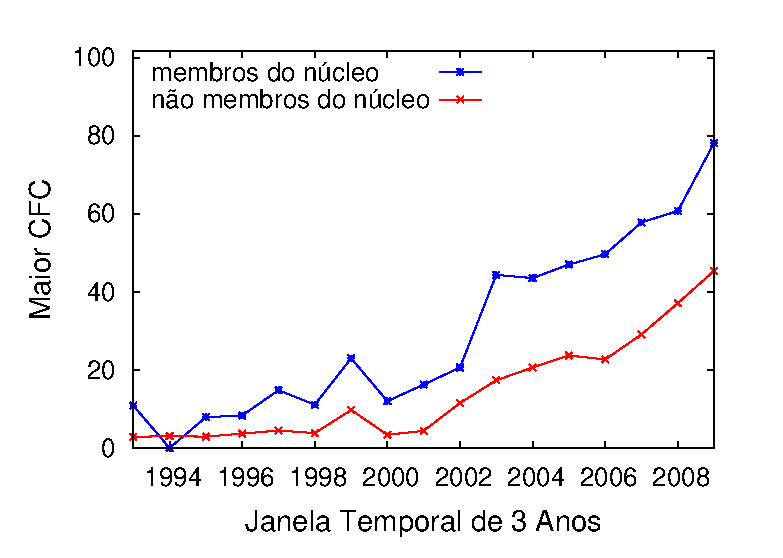
\includegraphics[scale=.6]{../graficos/core_over_time/core_community/pt_BR/acm_multimedia_janela_3_core_maior_componente_conectado.eps}
  }
  \subfloat[\textit{Betweenness} médio]{%
    \label{fig:core_com_acm_multimedia_betweenness_apendice}
    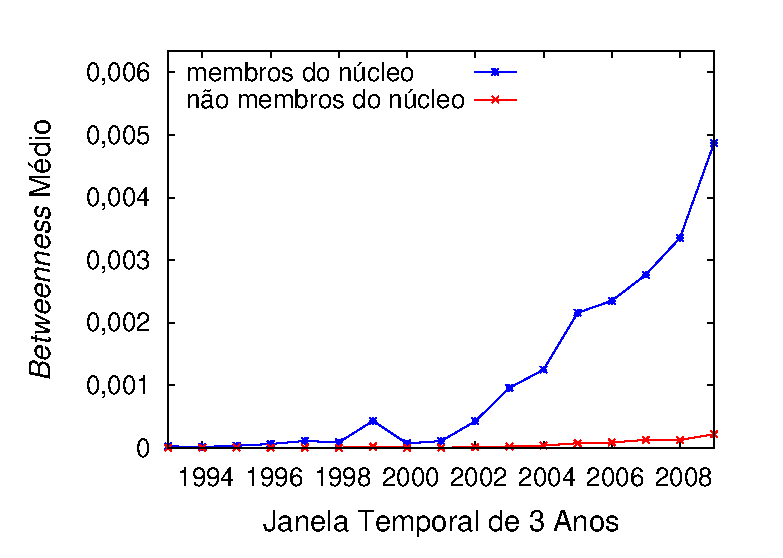
\includegraphics[scale=.6]{../graficos/core_over_time/core_community/pt_BR/acm_multimedia_janela_3_core_betweenness.eps}
  }
  \end{center}
  \caption{Propriedades da comunidade MM para os membros e não membros do núcleo}
  \label{fig:metrics_comparing_core_community_acm_multimedia_apendice}
\end{figure}

\begin{figure}[!htb]
  \begin{center}
  \subfloat[Coeficiente de agrupamento]{%
    \label{fig:core_com_mobicom_clustering_coefficient_apendice}
    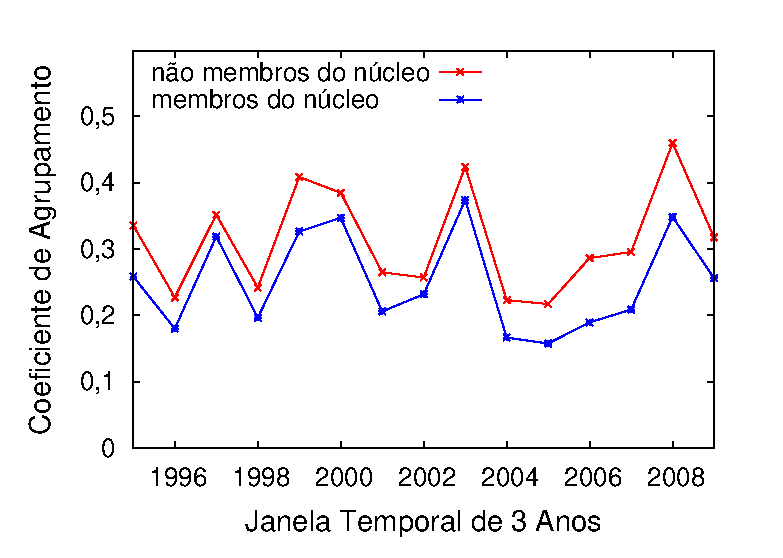
\includegraphics[scale=.6]{../graficos/core_over_time/core_community/pt_BR/mobicom_janela_3_core_coeficiente_agrupamento.eps}
  }
  \subfloat[Grau médio]{%
    \label{fig:core_com_mobicom_average_degree_apendice}
    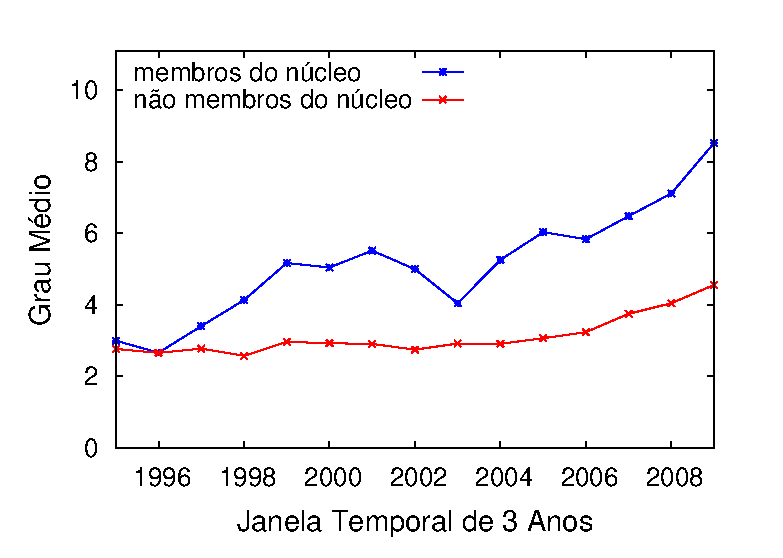
\includegraphics[scale=.6]{../graficos/core_over_time/core_community/pt_BR/mobicom_janela_3_core_grau_medio_nodos.eps}
  }
  \\
  \subfloat[Maior CFC]{%
    \label{fig:core_com_mobicom_largest_connected_component_apendice}
    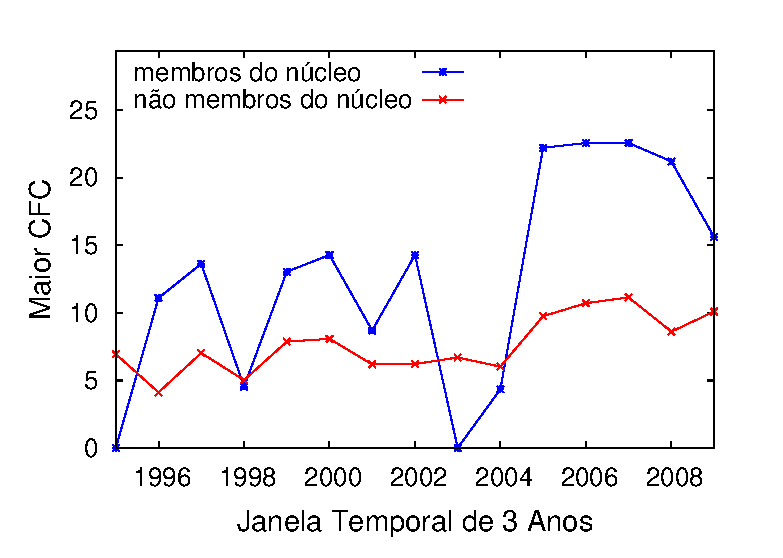
\includegraphics[scale=.6]{../graficos/core_over_time/core_community/pt_BR/mobicom_janela_3_core_maior_componente_conectado.eps}
  }
  \subfloat[\textit{Betweenness} médio]{%
    \label{fig:core_com_mobicom_betweenness_apendice}
    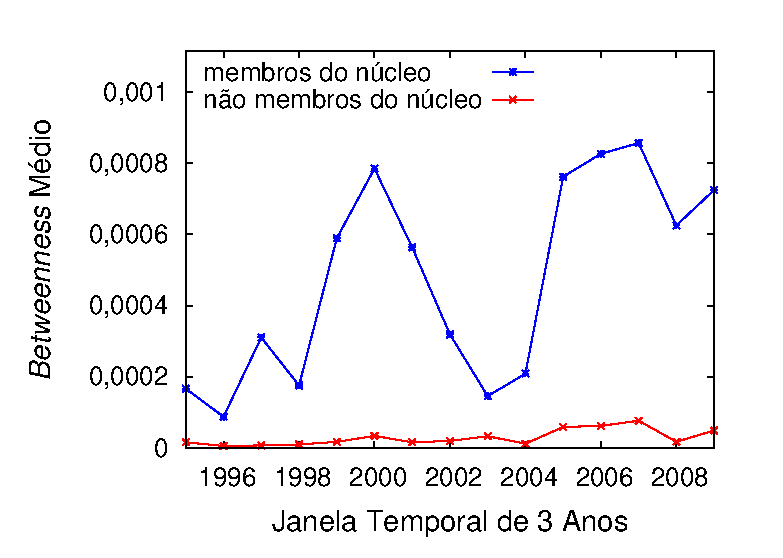
\includegraphics[scale=.6]{../graficos/core_over_time/core_community/pt_BR/mobicom_janela_3_core_betweenness.eps}
  }
  \end{center}
  \caption{Propriedades da comunidade MOBICOM para os membros e não membros do núcleo}
  \label{fig:metrics_comparing_core_community_mobicom_apendice}
\end{figure}

\begin{figure}[!htb]
  \begin{center}
  \subfloat[Coeficiente de agrupamento]{%
    \label{fig:core_com_podc_clustering_coefficient_apendice}
    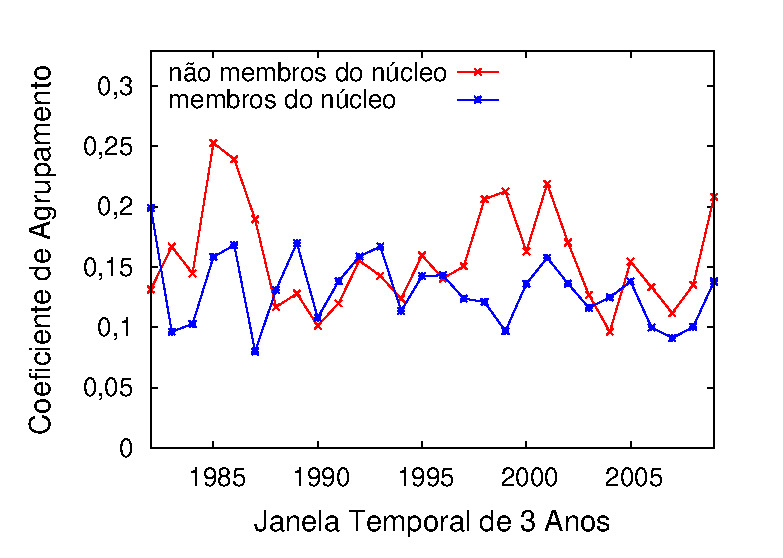
\includegraphics[scale=.6]{../graficos/core_over_time/core_community/pt_BR/podc_janela_3_core_coeficiente_agrupamento.eps}
  }
  \subfloat[Grau médio]{%
    \label{fig:core_com_podc_average_degree_apendice}
    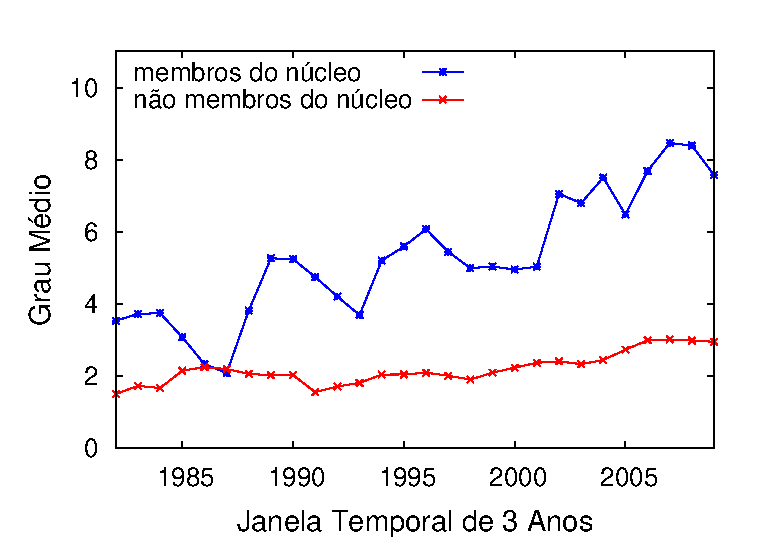
\includegraphics[scale=.6]{../graficos/core_over_time/core_community/pt_BR/podc_janela_3_core_grau_medio_nodos.eps}
  }
  \\
  \subfloat[Maior CFC]{%
    \label{fig:core_com_podc_largest_connected_component_apendice}
    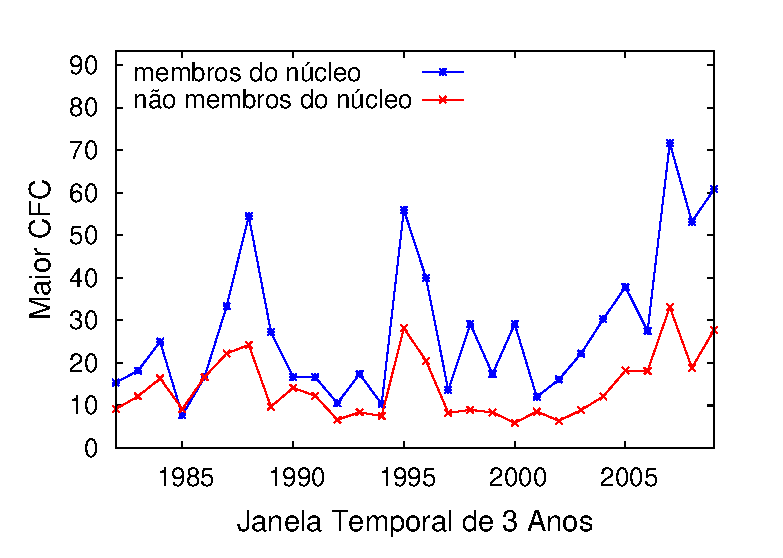
\includegraphics[scale=.6]{../graficos/core_over_time/core_community/pt_BR/podc_janela_3_core_maior_componente_conectado.eps}
  }
  \subfloat[\textit{Betweenness} médio]{%
    \label{fig:core_com_podc_betweenness_apendice}
    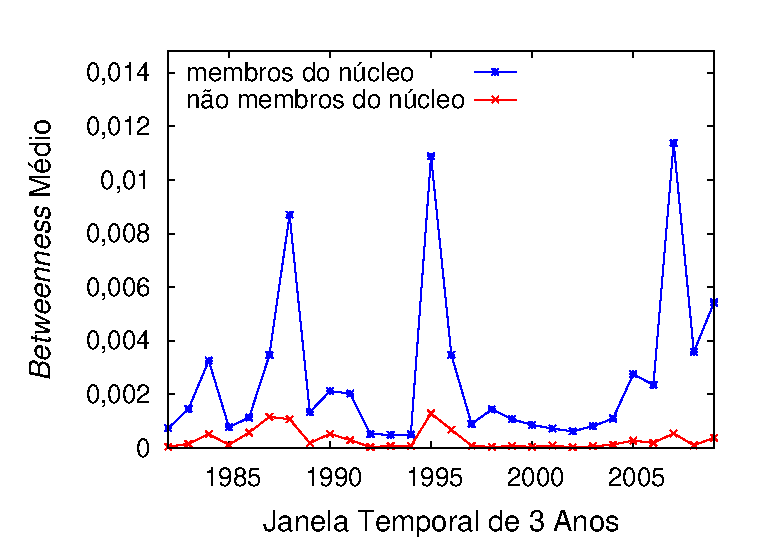
\includegraphics[scale=.6]{../graficos/core_over_time/core_community/pt_BR/podc_janela_3_core_betweenness.eps}
  }
  \end{center}
  \caption{Propriedades da comunidade PODC para os membros e não membros do núcleo}
  \label{fig:metrics_comparing_core_community_podc_apendice}
\end{figure}

\begin{figure}[!htb]
  \begin{center}
  \subfloat[Coeficiente de agrupamento]{%
    \label{fig:core_com_popl_clustering_coefficient_apendice}
    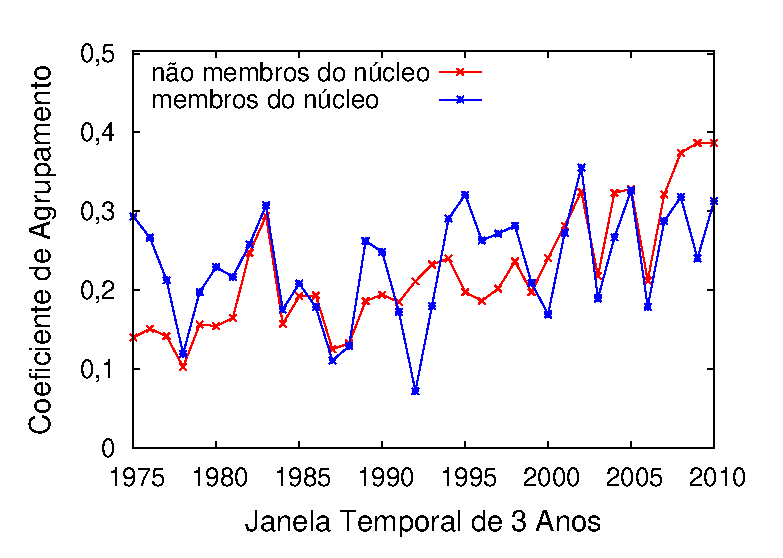
\includegraphics[scale=.6]{../graficos/core_over_time/core_community/pt_BR/popl_janela_3_core_coeficiente_agrupamento.eps}
  }
  \subfloat[Grau médio]{%
    \label{fig:core_com_popl_average_degree_apendice}
    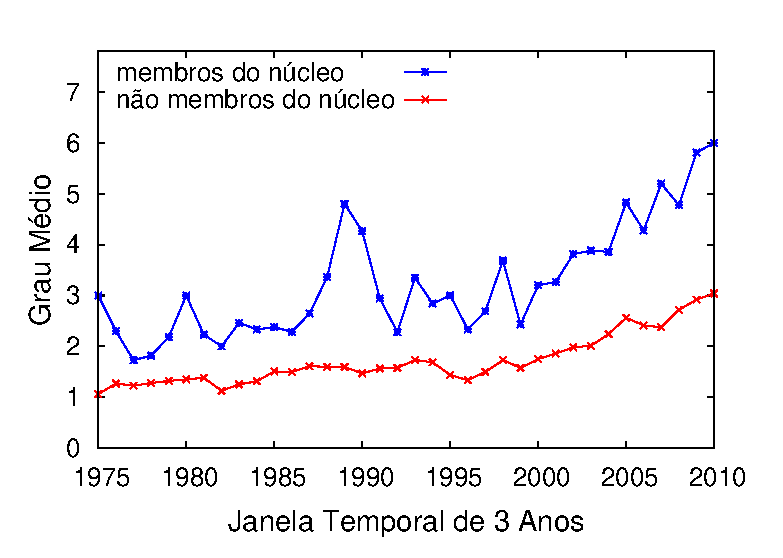
\includegraphics[scale=.6]{../graficos/core_over_time/core_community/pt_BR/popl_janela_3_core_grau_medio_nodos.eps}
  }
  \phantomcaption
  \end{center}
\end{figure}
\begin{figure}[!htb]
  \begin{center}
  \ContinuedFloat
  \subfloat[Maior CFC]{%
    \label{fig:core_com_popl_largest_connected_component_apendice}
    \includegraphics[scale=.6]{../graficos/core_over_time/core_community/pt_BR/popl_janela_3_core_maior_componente_conectado.eps}
  }
  \subfloat[\textit{Betweenness} médio]{%
    \label{fig:core_com_popl_betweenness_apendice}
    \includegraphics[scale=.6]{../graficos/core_over_time/core_community/pt_BR/popl_janela_3_core_betweenness.eps}
  }
  \end{center}
  \caption{Propriedades da comunidade POPL para os membros e não membros do núcleo}
  \label{fig:metrics_comparing_core_community_popl_apendice}
\end{figure}

\begin{figure}[!htb]
  \begin{center}
  \subfloat[Coeficiente de agrupamento]{%
    \label{fig:core_com_sac_clustering_coefficient_apendice}
    \includegraphics[scale=.6]{../graficos/core_over_time/core_community/pt_BR/sac_janela_3_core_coeficiente_agrupamento.eps}
  }
  \subfloat[Grau médio]{%
    \label{fig:core_com_sac_average_degree_apendice}
    \includegraphics[scale=.6]{../graficos/core_over_time/core_community/pt_BR/sac_janela_3_core_grau_medio_nodos.eps}
  }
  \\
  \subfloat[Maior CFC]{%
    \label{fig:core_com_sac_largest_connected_component_apendice}
    \includegraphics[scale=.6]{../graficos/core_over_time/core_community/pt_BR/sac_janela_3_core_maior_componente_conectado.eps}
  }
  \subfloat[\textit{Betweenness} médio]{%
    \label{fig:core_com_sac_betweenness_apendice}
    \includegraphics[scale=.6]{../graficos/core_over_time/core_community/pt_BR/sac_janela_3_core_betweenness.eps}
  }
  \end{center}
  \caption{Propriedades da comunidade SAC para os membros e não membros do núcleo}
  \label{fig:metrics_comparing_core_community_sac_apendice}
\end{figure}

\begin{figure}[!htb]
  \begin{center}
  \subfloat[Coeficiente de agrupamento]{%
    \label{fig:core_com_sigcomm_clustering_coefficient_apendice}
    \includegraphics[scale=.6]{../graficos/core_over_time/core_community/pt_BR/sigcomm_janela_3_core_coeficiente_agrupamento.eps}
  }
  \subfloat[Grau médio]{%
    \label{fig:core_com_sigcomm_average_degree_apendice}
    \includegraphics[scale=.6]{../graficos/core_over_time/core_community/pt_BR/sigcomm_janela_3_core_grau_medio_nodos.eps}
  }
  \\
  \subfloat[Maior CFC]{%
    \label{fig:core_com_sigcomm_largest_connected_component_apendice}
    \includegraphics[scale=.6]{../graficos/core_over_time/core_community/pt_BR/sigcomm_janela_3_core_maior_componente_conectado.eps}
  }
  \subfloat[\textit{Betweenness} médio]{%
    \label{fig:core_com_sigcomm_betweenness_apendice}
    \includegraphics[scale=.6]{../graficos/core_over_time/core_community/pt_BR/sigcomm_janela_3_core_betweenness.eps}
  }
  \end{center}
  \caption{Propriedades da comunidade SIGCOMM para os membros e não membros do núcleo}
  \label{fig:metrics_comparing_core_community_sigcomm_apendice}
\end{figure}

\begin{figure}[!htb]
  \begin{center}
  \subfloat[Coeficiente de agrupamento]{%
    \label{fig:core_com_sigcse_clustering_coefficient_apendice}
    \includegraphics[scale=.6]{../graficos/core_over_time/core_community/pt_BR/sigcse_janela_3_core_coeficiente_agrupamento.eps}
  }
  \subfloat[Grau médio]{%
    \label{fig:core_com_sigcse_average_degree_apendice}
    \includegraphics[scale=.6]{../graficos/core_over_time/core_community/pt_BR/sigcse_janela_3_core_grau_medio_nodos.eps}
  }
  \phantomcaption
  \end{center}
\end{figure}
\begin{figure}[!htb]
  \begin{center}
  \ContinuedFloat
  \subfloat[Maior CFC]{%
    \label{fig:core_com_sigcse_largest_connected_component_apendice}
    \includegraphics[scale=.6]{../graficos/core_over_time/core_community/pt_BR/sigcse_janela_3_core_maior_componente_conectado.eps}
  }
  \subfloat[\textit{Betweenness} médio]{%
    \label{fig:core_com_sigcse_betweenness_apendice}
    \includegraphics[scale=.6]{../graficos/core_over_time/core_community/pt_BR/sigcse_janela_3_core_betweenness.eps}
  }
  \end{center}
  \caption{Propriedades da comunidade SIGCSE para os membros e não membros do núcleo}
  \label{fig:metrics_comparing_core_community_sigcse_apendice}
\end{figure}

\begin{figure}[!htb]
  \begin{center}
  \subfloat[Coeficiente de agrupamento]{%
    \label{fig:core_com_sigdoc_clustering_coefficient_apendice}
    \includegraphics[scale=.6]{../graficos/core_over_time/core_community/pt_BR/sigdoc_janela_3_core_coeficiente_agrupamento.eps}
  }
  \subfloat[Grau médio]{%
    \label{fig:core_com_sigdoc_average_degree_apendice}
    \includegraphics[scale=.6]{../graficos/core_over_time/core_community/pt_BR/sigdoc_janela_3_core_grau_medio_nodos.eps}
  }
  \\
  \subfloat[Maior CFC]{%
    \label{fig:core_com_sigdoc_largest_connected_component_apendice}
    \includegraphics[scale=.6]{../graficos/core_over_time/core_community/pt_BR/sigdoc_janela_3_core_maior_componente_conectado.eps}
  }
  \subfloat[\textit{Betweenness} médio]{%
    \label{fig:core_com_sigdoc_betweenness_apendice}
    \includegraphics[scale=.6]{../graficos/core_over_time/core_community/pt_BR/sigdoc_janela_3_core_betweenness.eps}
  }
  \end{center}
  \caption{Propriedades da comunidade SIGDOC para os membros e não membros do núcleo}
  \label{fig:metrics_comparing_core_community_sigdoc_apendice}
\end{figure}

\begin{figure}[!htb]
  \begin{center}
  \subfloat[Coeficiente de agrupamento]{%
    \label{fig:core_com_siggraph_clustering_coefficient_apendice}
    \includegraphics[scale=.6]{../graficos/core_over_time/core_community/pt_BR/siggraph_janela_3_core_coeficiente_agrupamento.eps}
  }
  \subfloat[Grau médio]{%
    \label{fig:core_com_siggraph_average_degree_apendice}
    \includegraphics[scale=.6]{../graficos/core_over_time/core_community/pt_BR/siggraph_janela_3_core_grau_medio_nodos.eps}
  }
  \\
  \subfloat[Maior CFC]{%
    \label{fig:core_com_siggraph_largest_connected_component_apendice}
    \includegraphics[scale=.6]{../graficos/core_over_time/core_community/pt_BR/siggraph_janela_3_core_maior_componente_conectado.eps}
  }
  \subfloat[\textit{Betweenness} médio]{%
    \label{fig:core_com_siggraph_betweenness_apendice}
    \includegraphics[scale=.6]{../graficos/core_over_time/core_community/pt_BR/siggraph_janela_3_core_betweenness.eps}
  }
  \end{center}
  \caption{Propriedades da comunidade SIGGRAPH para os membros e não membros do núcleo}
  \label{fig:metrics_comparing_core_community_siggraph_apendice}
\end{figure}

\begin{figure}[!htb]
  \begin{center}
  \subfloat[Coeficiente de agrupamento]{%
    \label{fig:core_com_sigir_clustering_coefficient_apendice}
    \includegraphics[scale=.6]{../graficos/core_over_time/core_community/pt_BR/sigir_janela_3_core_coeficiente_agrupamento.eps}
  }
  \subfloat[Grau médio]{%
    \label{fig:core_com_sigir_average_degree_apendice}
    \includegraphics[scale=.6]{../graficos/core_over_time/core_community/pt_BR/sigir_janela_3_core_grau_medio_nodos.eps}
  }
  \phantomcaption
  \end{center}
\end{figure}
\begin{figure}[!htb]
  \begin{center}
  \ContinuedFloat
  \subfloat[Maior CFC]{%
    \label{fig:core_com_sigir_largest_connected_component_apendice}
    \includegraphics[scale=.6]{../graficos/core_over_time/core_community/pt_BR/sigir_janela_3_core_maior_componente_conectado.eps}
  }
  \subfloat[\textit{Betweenness} médio]{%
    \label{fig:core_com_sigir_betweenness_apendice}
    \includegraphics[scale=.6]{../graficos/core_over_time/core_community/pt_BR/sigir_janela_3_core_betweenness.eps}
  }
  \end{center}
  \caption{Propriedades da comunidade SIGIR para os membros e não membros do núcleo}
  \label{fig:metrics_comparing_core_community_sigir_apendice}
\end{figure}

\begin{figure}[!htb]
  \begin{center}
  \subfloat[Coeficiente de agrupamento]{%
    \label{fig:core_com_sigmetrics_clustering_coefficient_apendice}
    \includegraphics[scale=.6]{../graficos/core_over_time/core_community/pt_BR/sigmetrics_janela_3_core_coeficiente_agrupamento.eps}
  }
  \subfloat[Grau médio]{%
    \label{fig:core_com_sigmetrics_average_degree_apendice}
    \includegraphics[scale=.6]{../graficos/core_over_time/core_community/pt_BR/sigmetrics_janela_3_core_grau_medio_nodos.eps}
  }
  \\
  \subfloat[Maior CFC]{%
    \label{fig:core_com_sigmetrics_largest_connected_component_apendice}
    \includegraphics[scale=.6]{../graficos/core_over_time/core_community/pt_BR/sigmetrics_janela_3_core_maior_componente_conectado.eps}
  }
  \subfloat[\textit{Betweenness} médio]{%
    \label{fig:core_com_sigmetrics_betweenness_apendice}
    \includegraphics[scale=.6]{../graficos/core_over_time/core_community/pt_BR/sigmetrics_janela_3_core_betweenness.eps}
  }
  \end{center}
  \caption{Propriedades da comunidade SIGMETRICS para os membros e não membros do núcleo}
  \label{fig:metrics_comparing_core_community_sigmetrics_apendice}
\end{figure}

\begin{figure}[!htb]
  \begin{center}
  \subfloat[Coeficiente de agrupamento]{%
    \label{fig:core_com_stoc_clustering_coefficient_apendice}
    \includegraphics[scale=.6]{../graficos/core_over_time/core_community/pt_BR/stoc_janela_3_core_coeficiente_agrupamento.eps}
  }
  \subfloat[Grau médio]{%
    \label{fig:core_com_stoc_average_degree_apendice}
    \includegraphics[scale=.6]{../graficos/core_over_time/core_community/pt_BR/stoc_janela_3_core_grau_medio_nodos.eps}
  }
  \\
  \subfloat[Maior CFC]{%
    \label{fig:core_com_stoc_largest_connected_component_apendice}
    \includegraphics[scale=.6]{../graficos/core_over_time/core_community/pt_BR/stoc_janela_3_core_maior_componente_conectado.eps}
  }
  \subfloat[\textit{Betweenness} médio]{%
    \label{fig:core_com_stoc_betweenness_apendice}
    \includegraphics[scale=.6]{../graficos/core_over_time/core_community/pt_BR/stoc_janela_3_core_betweenness.eps}
  }
  \end{center}
  \caption{Propriedades da comunidade STOC para os membros e não membros do núcleo}
  \label{fig:metrics_comparing_core_community_stoc_apendice}
\end{figure}